\chapter{Organisation, vue d'ensemble}
\label{Chapter2}

Cette première phase de recherche a consisté à réfléchir à une architecture possible pour cette application. Comme discuté en introduction, l'objectif est de proposer une structure générale, modulaire. Ce faisant, il sera plus aisé d'étudier les possibilités offertes pour chaque "brique", dont l'assemblage donnera le résultat final.

Un \textit{Mind map} est une technique pratique pour explorer de multiples possibilités, surtout lorsque l'on a pas une idée précise. On l'effectue traditionnellement sur un tableau, souvent à plusieurs, en collaboration. Chacun peut alors développer une nouvelle branche, ou compléter une existante, et apporter sa contribution.
Cette méthode est aussi efficace lorsque l'on est seul, afin de structurer et réorganiser ses idées au gré de ses réflexions.
Parmi les outils informatiques existants, citons XMind\footnote{\url{https://www.xmind.net/}}, logiciel client très complet, multiplateforme et proposant une version gratuite, ainsi que Coggle\footnote{\url{https://coggle.it/}}, application web avec une formule gratuite également.

\begin{figure}
    \centering
    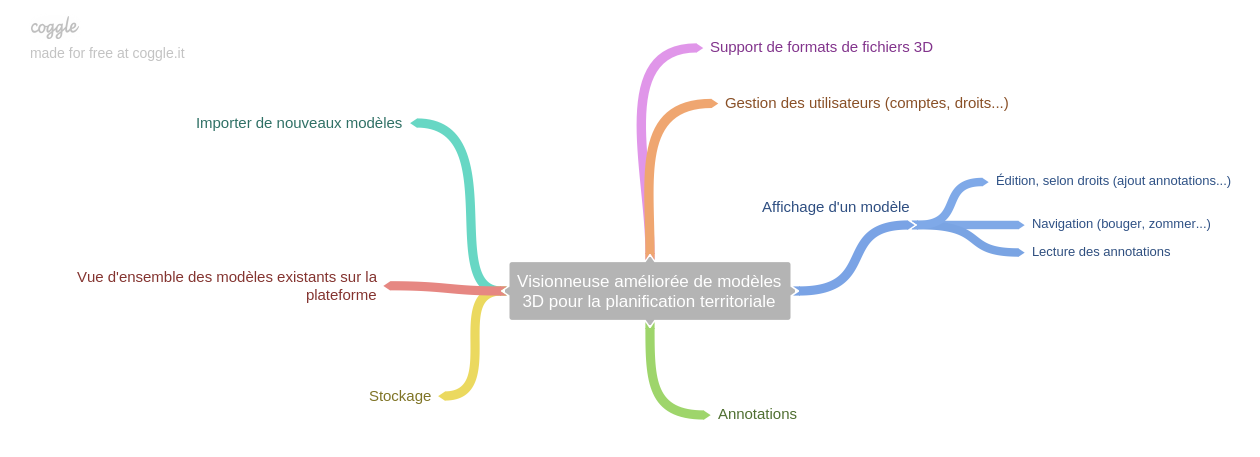
\includegraphics[width=\linewidth]{Figures/mip-viewer-mindmap.png}
    \caption{Résultat du \textit{Mind map} des modules imaginés pour l'application}
    \label{fig:mip-viewer-mindmap}
\end{figure}

\section{Cas d'utilisation, fonctionnalités imaginées}

Lors des séances préparatoires, M. Donzé a décrit des contextes d'utilisation possibles de la plateforme. Cela a permis d'identifier différentes catégories d'acteurs qui pourraient être amener à l'utiliser.

Prenons le cas d'un concours d'architecture :

- Les participants doivent pouvoir :
    - Télécharger la maquette d'origine sur laquelle ils devront se baser (par exemple un plan localisé de quartier dans son état actuel).
    - Déposer leur version modifiée de la maquette; il faudrait éventuellement que le système vérifie que celle-ci remplisse les critères, que tous les éléments ont bien été rendus...

- Des experts doivent pouvoir :
    - Vérifier que les propositions répondent à certains critères (effectuer une espèce de préselection)
    
- Le jury - les personnes qui jugent - doivent avoir une vue plus générale

- Public, personnes qui vont consulter les résultats (cadre restreint, service de l'urbanisme par exemple)

- Une fois les résultats publiés (jugement effectué), peut être montré au grand public (exposition)

Fonctionnalités :
	- pouvoir récupérer modèles
	- déposer modèles
	- pouvoir annoter (annotation localisée). Deux types d'annotation :
		- Annotation du bureau d'architectures
		    - Concurrent devrait pouvoir proposer des vues prédéfinies de leur projet p.ex.
		- Annotation genre questions que le jury se pose sur un point
Annotation  destinée au grand public

\begin{figure}
    \centering
    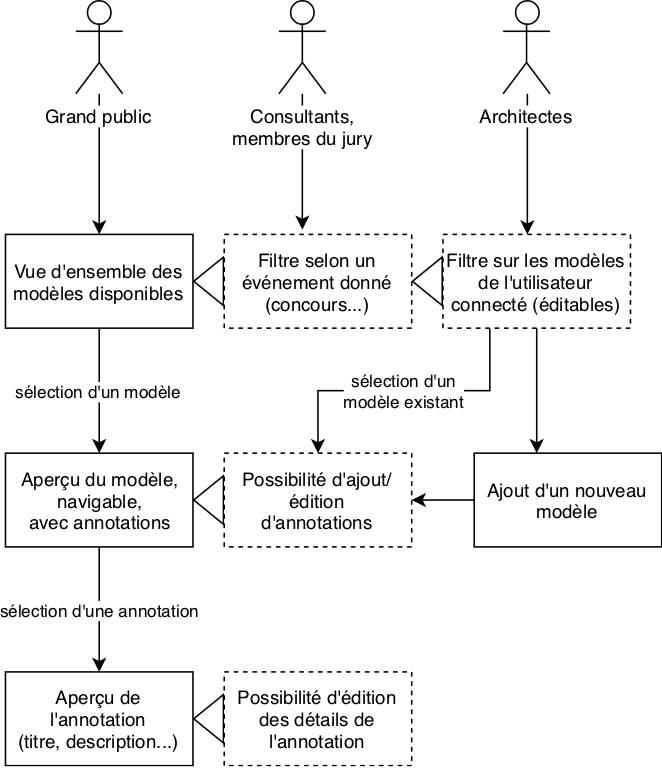
\includegraphics[width=0.8\linewidth]{Figures/use-cases.png}
    \caption{Exemples de cas d'utilisation}
    \label{fig:use-cases}
\end{figure}

Annotations : vue 360
naviguer dans une animation ? exemple : projet à plusieurs années d’intervalle, pouvoir bouger sur un curseur






